% ********** Rozdział 4 **********
\chapter{Harmonogram realizacji projektu}

\section{Harmonogram realizacji}

W celu zaplanowania i monitorowania postępów w realizacji projektu został stworzony diagram Gantta, który przedstawia podział projektu na poszczególne etapy i terminy ich realizacji. Diagram ten jest przedstawiony na rysunku \ref{fig:gantt}.

\begin{figure}[h!]
    \centering
    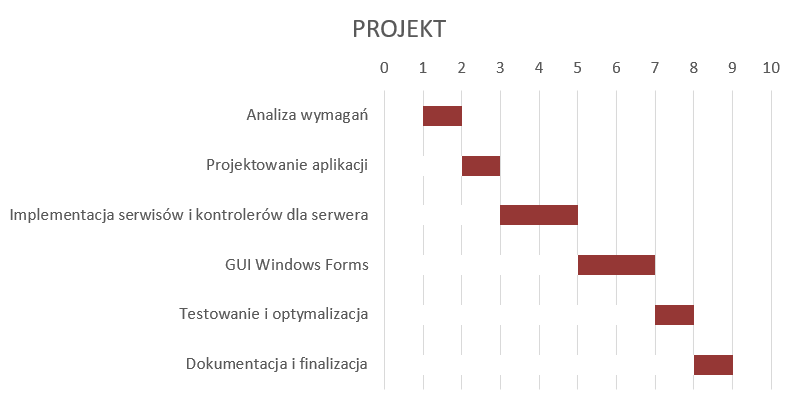
\includegraphics[width=\textwidth]{figures/diagram.png}
    \caption{Diagram Gantta przedstawiający harmonogram realizacji projektu.}
    \label{fig:gantt}
\end{figure}

Diagram obejmuje następujące etapy:
\begin{enumerate}
    \item \textbf{Analiza wymagań (tygodnie 1-2):} Na tym etapie zebrano wymagania i przygotowano ogólną koncepcję projektu.
    \item \textbf{Projektowanie aplikacji (tygodnie 2-3):} Opracowano architekturę systemu, w tym schematy baz danych i strukturę kodu.
    \item \textbf{Implementacja serwisów i kontrolerów dla serwera (tygodnie 3-5):} Zaimplementowano backend aplikacji z wykorzystaniem API.
    \item \textbf{GUI Windows Forms (tygodnie 5-7):} Stworzono graficzny interfejs użytkownika, umożliwiający interakcję z systemem.
    \item \textbf{Testowanie i optymalizacja (tygodnie 7-8):} Przeprowadzono testy jednostkowe i integracyjne, wprowadzono poprawki oraz zoptymalizowano kod.
    \item \textbf{Dokumentacja i finalizacja (tygodnie 8-9):} Przygotowano dokumentację użytkownika i kodu oraz sfinalizowano projekt.
\end{enumerate}

\section{Repozytorium i system kontroli wersji}

Kod źródłowy projektu został umieszczony w publicznie dostępnym repozytorium na platformie GitHub. Repozytorium dostępne jest pod adresem w załączniku.


W projekcie wykorzystano system kontroli wersji \textbf{Git}, który umożliwia:
\begin{itemize}
    \item Śledzenie historii zmian w kodzie.
    \item Współpracę zespołową poprzez rozgałęzienia (\textit{branches}) i scalanie (\textit{merge}).
    \item Szybkie cofanie wprowadzonych zmian w przypadku wykrycia błędów.
\end{itemize}

\textbf{Struktura repozytorium:}  
Struktura repozytorium odpowiada strukturze projektu opisanej w poprzednich rozdziałach

% ********** Koniec rozdziału **********